\section{Métodos de interpolación}
\label{sec:cap2-metodos-interpolacion}

La interpolación espacial, consiste en la utilización de puntos con valores conocidos, también denominados puntos
de control, para estimar una variable en lugares donde se desconoce; también se considera una forma de transformar
información puntual en información de superficie, con el objetivo de combinarla con otros datos para facilitar el
análisis y la modelado espacial.

Todos los métodos de interpolación se basan en la presunción lógica de que cuanto más cercanos están dos puntos
sobre la superficie terrestre, los valores de cualquier variable cuantitativa que midamos en ellos serán más
parecidos, para expresarlo más técnicamente, las variables espaciales muestran autocorrelación espacial \cite{fAlonsoSig2006}.

El resultado de la interpolación espacial depende de un algoritmo computacional o una ecuación matemática en la
cual se emplean los datos de los puntos de control\cite{NINO2011}.


\subsection {Red de Triángulos Irregulares (TIN)}
Las Redes Irregulares de Triángulos (TIN por sus siglas en ingles Triangulated Irregular Network), se generan a
partir de valores puntuales tratando de conseguir triángulos que maximicen la relación área/perímetro, el conjunto
de todos los triángulos forma un objeto geométrico denominado conjunto convexo\cite{fAlonsoSig2006}. Son
ampliamente utilizados como método para la representación de modelos de elevaciones, ya que producen resultados
visualmente muy buenos, sin embargo a la hora de realizar la integración con la información raster restante, se
necesita interpolar una capa raster a partir de los triángulos.

Según \cite{cPachecoMDE2003} TIN utiliza los puntos de entrada para construir una red de triángulos según el
criterio de Delauny: en cada triángulo, el círculo que pasa a través de los tres vértices no encierra ningún otro
punto de entrada (el criterio de Delauny genera, tanto como le es posible, triángulos pequeños y equiláteros y es
ley ser utilizado para crear objetos TIN). Luego, el proceso ajusta una superficie plana a cada triángulo, de
manera tal que el total de la superficie está modelada como una colección de facetas trianguladas planas.


\begin{figure}
\centering
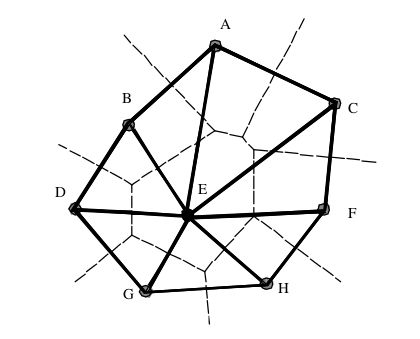
\includegraphics[width=0.4\textwidth]{capitulo-2/graphics/TIN-cPachecoMDE2003.png}
\caption{\label{fig:sig-tin}Red de Triángulos Irregulares (TIN) (Tomado de \cite{cPachecoMDE2003}).}
\end{figure}


\subsection{Ponderación de la inversa de la distancia (IDW)}
Estima los puntos del modelo realizando una asignación de pesos a los datos del entorno en función inversa a la
distancia que los separa del punto en cuestión. De esta forma, se acepta que los puntos más próximos al centroide
intervienen de manera más relevante en la obtención del valor definitivo de Z para ese punto.

La elección del exponente de ponderación(p) determina la contribución de los puntos circundantes al punto 
problema, cuanto mayor es p, más contribuyen los puntos próximos. Es necesario contar con muchos puntos para la
interpolación.

La forma general de encontrar un valor interpolado $u$ en un punto $x$ basado en muestras $u_i = u (x_i)$ para 
$i = 0,1, ..., N$ utilizando IDW es una función de interpolación:

\begin{equation}\label{eq:interpolacion-idw}
 u(x) = \sum_{i=1}^{N} \frac{w_i(X)}{\sum_{j=1}^{N} w_j(X)}
\end{equation}

donde 

\begin{equation} 
w_i(X) =  \frac{1}{d(X, X_i)^p} 
\end{equation}

\subsection{Kriging}
El Kriging es un método geoestadístico de interpolación espacial de carácter global, exacto y estocástico. La 
idea básica de este método corresponde a la noción de dependencia espacial, según la cual las muestras cercanas
tienen mayor similitud entre sí que las más apartadas\cite{NINO2011}.

Se presenta con un método de interpolación con una expresión general similar a la anterior (IDW). La diferencia
básica es que asume que la altitud puede definirse como una variable regionalizada. Supone que la variación
espacial de la variable a representar puede ser explicada al menos parcialmente mediante funciones de correlación
espacial(la variación espacial de los valores de z puede deducirse de los valores circundantes de acuerdo con unas
funciones homogéneas en toda el área).
